% Created by tikzDevice version 0.6.2-92-0ad2792 on 2013-03-05 17:06:53
% !TEX encoding = UTF-8 Unicode
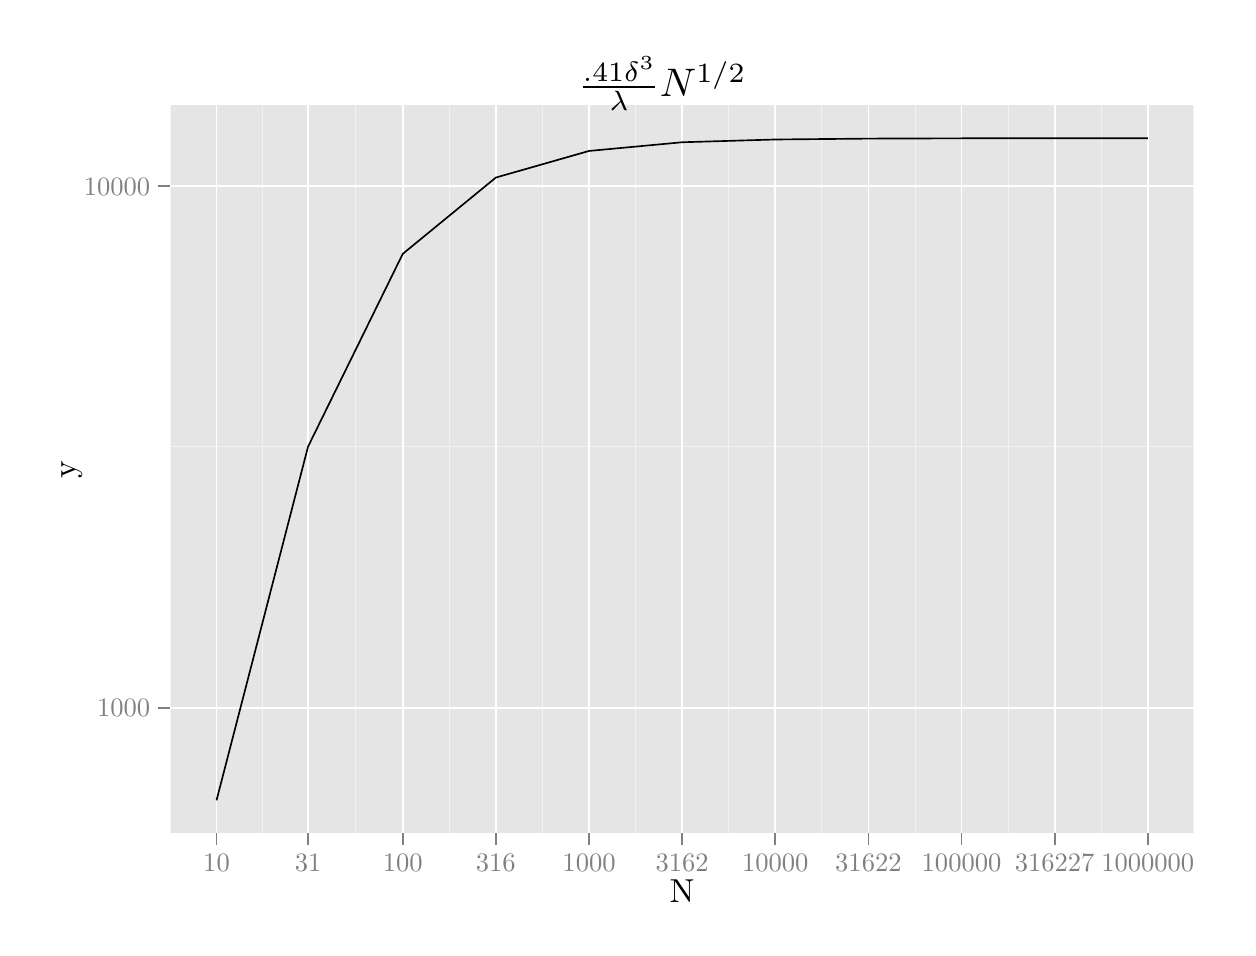
\begin{tikzpicture}[x=1pt,y=1pt]
\definecolor[named]{fillColor}{rgb}{1.00,1.00,1.00}
\path[use as bounding box,fill=fillColor,fill opacity=0.00] (0,0) rectangle (433.62,325.21);
\begin{scope}
\path[clip] (  0.00,  0.00) rectangle (433.62,325.21);
\definecolor[named]{drawColor}{rgb}{1.00,1.00,1.00}
\definecolor[named]{fillColor}{rgb}{1.00,1.00,1.00}

\path[draw=drawColor,line width= 0.6pt,line join=round,line cap=round,fill=fillColor] (  0.00,  0.00) rectangle (433.62,325.21);
\end{scope}
\begin{scope}
\path[clip] ( 51.42, 34.03) rectangle (421.57,297.23);
\definecolor[named]{fillColor}{rgb}{0.90,0.90,0.90}

\path[fill=fillColor] ( 51.42, 34.03) rectangle (421.57,297.23);
\definecolor[named]{drawColor}{rgb}{0.95,0.95,0.95}

\path[draw=drawColor,line width= 0.3pt,line join=round] ( 51.42,173.75) --
	(421.57,173.75);

\path[draw=drawColor,line width= 0.3pt,line join=round] ( 51.71, 34.03) --
	( 51.71,297.23);

\path[draw=drawColor,line width= 0.3pt,line join=round] ( 84.78, 34.03) --
	( 84.78,297.23);

\path[draw=drawColor,line width= 0.3pt,line join=round] (118.43, 34.03) --
	(118.43,297.23);

\path[draw=drawColor,line width= 0.3pt,line join=round] (152.36, 34.03) --
	(152.36,297.23);

\path[draw=drawColor,line width= 0.3pt,line join=round] (186.01, 34.03) --
	(186.01,297.23);

\path[draw=drawColor,line width= 0.3pt,line join=round] (219.67, 34.03) --
	(219.67,297.23);

\path[draw=drawColor,line width= 0.3pt,line join=round] (253.32, 34.03) --
	(253.32,297.23);

\path[draw=drawColor,line width= 0.3pt,line join=round] (286.97, 34.03) --
	(286.97,297.23);

\path[draw=drawColor,line width= 0.3pt,line join=round] (320.62, 34.03) --
	(320.62,297.23);

\path[draw=drawColor,line width= 0.3pt,line join=round] (354.27, 34.03) --
	(354.27,297.23);

\path[draw=drawColor,line width= 0.3pt,line join=round] (387.92, 34.03) --
	(387.92,297.23);

\path[draw=drawColor,line width= 0.3pt,line join=round] (421.28, 34.03) --
	(421.28,297.23);
\definecolor[named]{drawColor}{rgb}{1.00,1.00,1.00}

\path[draw=drawColor,line width= 0.6pt,line join=round] ( 51.42, 79.45) --
	(421.57, 79.45);

\path[draw=drawColor,line width= 0.6pt,line join=round] ( 51.42,268.04) --
	(421.57,268.04);

\path[draw=drawColor,line width= 0.6pt,line join=round] ( 68.24, 34.03) --
	( 68.24,297.23);

\path[draw=drawColor,line width= 0.6pt,line join=round] (101.31, 34.03) --
	(101.31,297.23);

\path[draw=drawColor,line width= 0.6pt,line join=round] (135.54, 34.03) --
	(135.54,297.23);

\path[draw=drawColor,line width= 0.6pt,line join=round] (169.17, 34.03) --
	(169.17,297.23);

\path[draw=drawColor,line width= 0.6pt,line join=round] (202.85, 34.03) --
	(202.85,297.23);

\path[draw=drawColor,line width= 0.6pt,line join=round] (236.49, 34.03) --
	(236.49,297.23);

\path[draw=drawColor,line width= 0.6pt,line join=round] (270.15, 34.03) --
	(270.15,297.23);

\path[draw=drawColor,line width= 0.6pt,line join=round] (303.80, 34.03) --
	(303.80,297.23);

\path[draw=drawColor,line width= 0.6pt,line join=round] (337.45, 34.03) --
	(337.45,297.23);

\path[draw=drawColor,line width= 0.6pt,line join=round] (371.10, 34.03) --
	(371.10,297.23);

\path[draw=drawColor,line width= 0.6pt,line join=round] (404.75, 34.03) --
	(404.75,297.23);
\definecolor[named]{drawColor}{rgb}{0.00,0.00,0.00}

\path[draw=drawColor,line width= 0.6pt,line join=round] ( 68.24, 46.00) --
	(101.31,173.81) --
	(135.54,243.48) --
	(169.17,271.04) --
	(202.85,280.66) --
	(236.49,283.80) --
	(270.15,284.80) --
	(303.80,285.12) --
	(337.45,285.22) --
	(371.10,285.26) --
	(404.75,285.27);
\end{scope}
\begin{scope}
\path[clip] (  0.00,  0.00) rectangle (433.62,325.21);
\definecolor[named]{drawColor}{rgb}{0.50,0.50,0.50}

\node[text=drawColor,anchor=base east,inner sep=0pt, outer sep=0pt, scale=  0.96] at ( 44.30, 76.15) {1000};

\node[text=drawColor,anchor=base east,inner sep=0pt, outer sep=0pt, scale=  0.96] at ( 44.30,264.74) {10000};
\end{scope}
\begin{scope}
\path[clip] (  0.00,  0.00) rectangle (433.62,325.21);
\definecolor[named]{drawColor}{rgb}{0.50,0.50,0.50}

\path[draw=drawColor,line width= 0.6pt,line join=round] ( 47.15, 79.45) --
	( 51.42, 79.45);

\path[draw=drawColor,line width= 0.6pt,line join=round] ( 47.15,268.04) --
	( 51.42,268.04);
\end{scope}
\begin{scope}
\path[clip] (  0.00,  0.00) rectangle (433.62,325.21);
\definecolor[named]{drawColor}{rgb}{0.50,0.50,0.50}

\path[draw=drawColor,line width= 0.6pt,line join=round] ( 68.24, 29.77) --
	( 68.24, 34.03);

\path[draw=drawColor,line width= 0.6pt,line join=round] (101.31, 29.77) --
	(101.31, 34.03);

\path[draw=drawColor,line width= 0.6pt,line join=round] (135.54, 29.77) --
	(135.54, 34.03);

\path[draw=drawColor,line width= 0.6pt,line join=round] (169.17, 29.77) --
	(169.17, 34.03);

\path[draw=drawColor,line width= 0.6pt,line join=round] (202.85, 29.77) --
	(202.85, 34.03);

\path[draw=drawColor,line width= 0.6pt,line join=round] (236.49, 29.77) --
	(236.49, 34.03);

\path[draw=drawColor,line width= 0.6pt,line join=round] (270.15, 29.77) --
	(270.15, 34.03);

\path[draw=drawColor,line width= 0.6pt,line join=round] (303.80, 29.77) --
	(303.80, 34.03);

\path[draw=drawColor,line width= 0.6pt,line join=round] (337.45, 29.77) --
	(337.45, 34.03);

\path[draw=drawColor,line width= 0.6pt,line join=round] (371.10, 29.77) --
	(371.10, 34.03);

\path[draw=drawColor,line width= 0.6pt,line join=round] (404.75, 29.77) --
	(404.75, 34.03);
\end{scope}
\begin{scope}
\path[clip] (  0.00,  0.00) rectangle (433.62,325.21);
\definecolor[named]{drawColor}{rgb}{0.50,0.50,0.50}

\node[text=drawColor,anchor=base,inner sep=0pt, outer sep=0pt, scale=  0.96] at ( 68.24, 20.31) {10};

\node[text=drawColor,anchor=base,inner sep=0pt, outer sep=0pt, scale=  0.96] at (101.31, 20.31) {31};

\node[text=drawColor,anchor=base,inner sep=0pt, outer sep=0pt, scale=  0.96] at (135.54, 20.31) {100};

\node[text=drawColor,anchor=base,inner sep=0pt, outer sep=0pt, scale=  0.96] at (169.17, 20.31) {316};

\node[text=drawColor,anchor=base,inner sep=0pt, outer sep=0pt, scale=  0.96] at (202.85, 20.31) {1000};

\node[text=drawColor,anchor=base,inner sep=0pt, outer sep=0pt, scale=  0.96] at (236.49, 20.31) {3162};

\node[text=drawColor,anchor=base,inner sep=0pt, outer sep=0pt, scale=  0.96] at (270.15, 20.31) {10000};

\node[text=drawColor,anchor=base,inner sep=0pt, outer sep=0pt, scale=  0.96] at (303.80, 20.31) {31622};

\node[text=drawColor,anchor=base,inner sep=0pt, outer sep=0pt, scale=  0.96] at (337.45, 20.31) {100000};

\node[text=drawColor,anchor=base,inner sep=0pt, outer sep=0pt, scale=  0.96] at (371.10, 20.31) {316227};

\node[text=drawColor,anchor=base,inner sep=0pt, outer sep=0pt, scale=  0.96] at (404.75, 20.31) {1000000};
\end{scope}
\begin{scope}
\path[clip] (  0.00,  0.00) rectangle (433.62,325.21);
\definecolor[named]{drawColor}{rgb}{0.00,0.00,0.00}

\node[text=drawColor,anchor=base,inner sep=0pt, outer sep=0pt, scale=  1.20] at (236.50,  9.03) {N};
\end{scope}
\begin{scope}
\path[clip] (  0.00,  0.00) rectangle (433.62,325.21);
\definecolor[named]{drawColor}{rgb}{0.00,0.00,0.00}

\node[text=drawColor,rotate= 90.00,anchor=base,inner sep=0pt, outer sep=0pt, scale=  1.20] at ( 17.30,165.63) {y};
\end{scope}
\begin{scope}
\path[clip] (  0.00,  0.00) rectangle (433.62,325.21);
\definecolor[named]{drawColor}{rgb}{0.00,0.00,0.00}

\node[text=drawColor,anchor=base,inner sep=0pt, outer sep=0pt, scale=  1.44] at (236.50,300.24) {$\frac{.41\delta^3}{\lambda}N^{1/2}\quad $};
\end{scope}
\end{tikzpicture}
